\documentclass[12pt]{article}
%\usepackage[T1]{fontenc}
\usepackage{cite}
\usepackage[letterpaper,left=1in,right=1in,top=1in,bottom=1in]{geometry}
\setlength{\parindent}{15pt} % Default is 15pt.
\usepackage{setspace}
\usepackage{courier}
\usepackage{enumitem}
\usepackage{amsmath}
\usepackage{graphicx}
\usepackage{placeins}
%\onehalfspacing
\usepackage{color}

\pretolerance=10000
\tolerance=2000 
\emergencystretch=10pt

\usepackage{listings}
\definecolor{mygreen}{rgb}{0,0.6,0}
\definecolor{mygray}{rgb}{0.5,0.5,0.5}
\definecolor{mymauve}{rgb}{0.58,0,0.82}

\lstset{ %
	backgroundcolor=\color{white},   % choose the background color; you must add \usepackage{color} or \usepackage{xcolor}
	basicstyle=\scriptsize,        % the size of the fonts that are used for the code
	breakatwhitespace=false,         % sets if automatic breaks should only happen at whitespace
	breaklines=true,                 % sets automatic line breaking
	captionpos=b,                    % sets the caption-position to bottom
	commentstyle=\color{mygreen},    % comment style
	deletekeywords={...},            % if you want to delete keywords from the given language
	escapeinside={\%*}{*)},          % if you want to add LaTeX within your code
	extendedchars=true,              % lets you use non-ASCII characters; for 8-bits encodings only, does not work with UTF-8
	frame=single,                    % adds a frame around the code
	keepspaces=true,                 % keeps spaces in text, useful for keeping indentation of code (possibly needs columns=flexible)
	keywordstyle=\color{blue},       % keyword style
	language=Octave,                 % the language of the code
	morekeywords={*,...},            % if you want to add more keywords to the set
	numbers=left,                    % where to put the line-numbers; possible values are (none, left, right)
	numbersep=5pt,                   % how far the line-numbers are from the code
	numberstyle=\tiny\color{mygray}, % the style that is used for the line-numbers
	rulecolor=\color{black},         % if not set, the frame-color may be changed on line-breaks within not-black text (e.g. comments (green here))
	showspaces=false,                % show spaces everywhere adding particular underscores; it overrides 'showstringspaces'
	showstringspaces=false,          % underline spaces within strings only
	showtabs=false,                  % show tabs within strings adding particular underscores
	stepnumber=2,                    % the step between two line-numbers. If it's 1, each line will be numbered
	stringstyle=\color{mymauve},     % string literal style
	tabsize=2,                       % sets default tabsize to 2 spaces
}

\begin{document}
	
	\title{CS 5220: Homework 2}
	\date{\today}
	\author{Group 19: Robert Carson (rac428), Robert Chiodi (rmc298), Sam Tung (sat83)}
	\maketitle
		
	\section{Initial Profiling}
	In order to perform initial profiling of the code before any improvements are made, Intel's VTUNE was used via the terminal command line on Totient. In an attempt to get the most accurate results (taken with a large sample size), we decided to gather data while running the large wave simulation, invoked with the command \texttt{make big}. Information collected from VTUNE's ``advanced-hotspots'' option is used in our analysis.
		\subsection{Whole Program - Advanced Hotspots}
		First, hotspots in the entire program were examined in order to determine where our efforts should be directed. The time taken in the top 10 most time consuming functions can be seen below in Figure~\ref{top10}. Of these, it is clear that most of our optimization efforts should be directed to the functions \texttt{limited\_derivs}, \texttt{compute\_step}, and \texttt{compute\_fg\_speeds}. These functions were then examined individually, once again using VTUNE on our advanced-hotspots collection.
		\begin{figure}[h!]
			\begin{center}
				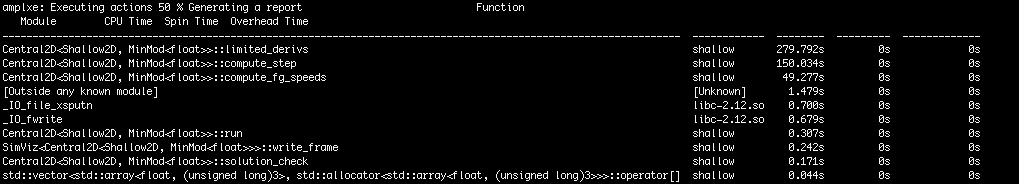
\includegraphics[width=0.7\columnwidth]{top10}
				\caption{Top 10 most time consuming functions in the wave simulation. Generated using Intel's VTUNE on Totient.}
				\label{top10}
			\end{center}
		\end{figure}
		\subsection{\texttt{limited\_derivs} - Advanced Hotspots}
		The function \texttt{limited\_deriv} is used to calculate the fluxes into and out of each cell in order to advance to the next time step. This involves a three point computational stencil in each direction and loops through the entire domain interior (the whole domain except for those where boundary conditions are applied). Each point requires $\mathtt{du.size()}\times 9$ floating point operations as well as $\mathtt{du.size()} \times 2$ calls to the intrinsic function $\mathtt{min}$. Sadly, the hotspot analysis on the \texttt{limited\_deriv} function, shown in Figure~\ref{init_lim_deriv}, does not give any hints on possible optimizations or bottle necks.
		
		\begin{figure}[h!]
			\begin{center}
				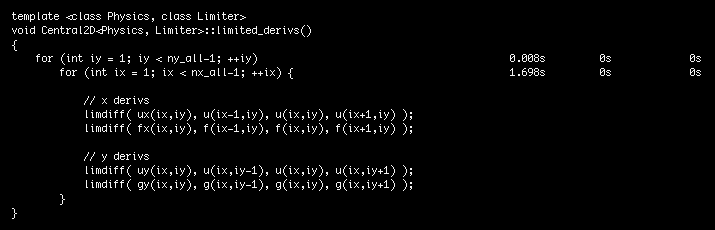
\includegraphics[width=0.7\columnwidth]{init_lim_deriv}
				\caption{Time taken to perform each loop present in \texttt{limited\_derivs}, recorded in core-seconds.}
				\label{init_lim_deriv}
			\end{center}
		\end{figure}
		
		\subsection{\texttt{compute\_step} - Advanced Hotspots}
		The purpose of \texttt{compute\_step} is to update the wave equation to the next time step using a predictor-corrector method. First, the fluxes are calculated in the prediction. Next, the corrector step uses the predicted fluxes, the differences in velocities, and the current velocities, to advance to the next time state. Luckily, VTUNE's report is more helpful than in the previous case, and provides extensive timings for this function, shown in Figure~\ref{init_compute_step}. The calculation in the corrector step can be seen as the most expensive cost of the function. It is important to note, however, that the predictor step and copying of the solution to the \texttt{u} array sum to half of the function's cost.
		\begin{figure}[h!]
			\begin{center}
				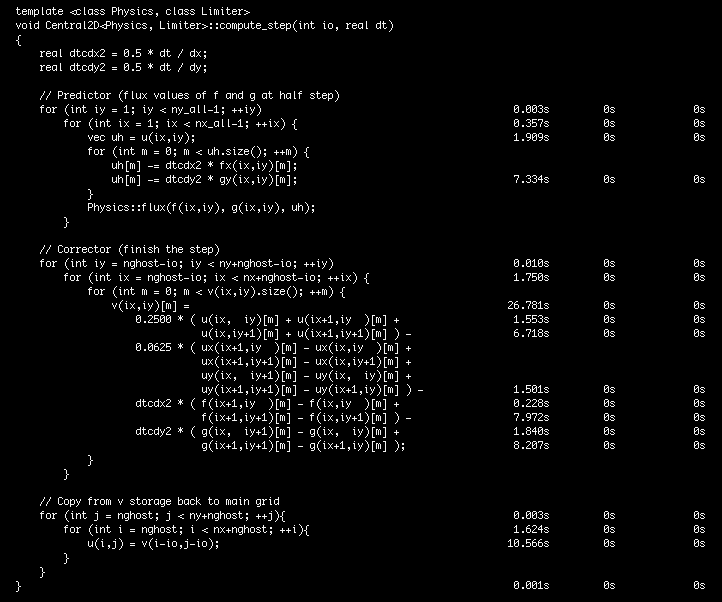
\includegraphics[width=0.7\columnwidth]{init_compute_step}
				\caption{Time taken to perform each loop present in \texttt{compute\_step}, recorded in core-seconds.}
				\label{init_compute_step}
			\end{center}
		\end{figure}	
		
		\subsection{\texttt{compute\_fg\_speeds} - Advanced Hotspots}
		The function of \texttt{compute\_fg\_speeds} has two primary responsibilities: to update the cell centered fluxes, \texttt{f} and \texttt{g}, and to calculate the maximum speed in the domain, allowing dynamic adjustment of the time step in order to satisfy the CFL condition and ensure numerical stability. The timing data for this function can be seen in Figure~\ref{init_compute_fg_speeds}. While the most time consuming portion of the code is most likely the calculation of the fluxes and wave speed (both of which are in the \texttt{Shallow2d} structure), the calls to the intrinsic function \texttt{max} also represent a non-trivial amount of time. 	
		\begin{figure}[h]
			\begin{center}
				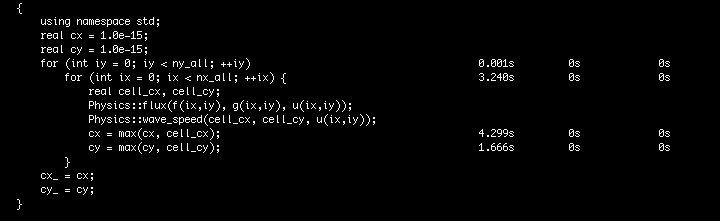
\includegraphics[width=0.7\columnwidth]{init_compute_fg_speeds}
				\caption{Time taken to perform each loop present in \texttt{compute\_fg\_speeds}, recorded in core-seconds.}
				\label{init_compute_fg_speeds}
			\end{center}
		\end{figure}	
		
		\FloatBarrier
	\section{Parallelization}
	While we are aware that the optimal programming of this code will not wholly be due to parallelization by OpenMP, it is most certainly necessary. Furthermore, future tuning and optimization of the code may change depending on whether the code is run in serial or parallel. For these reasons, we first decided to parallelize the code and compare its performance against the initial, serial code.
		\subsection{Naive Implementation of OpenMP}
		First, a naive implementation of OpenMP using pragmas was used. This involved placing \texttt{\#pragma omp parallel for} in front of the start of each for loop in the functions \texttt{init}, \texttt{apply\_periodic}, \texttt{compute\_fg\_speeds}, \texttt{limited\_derivs}, and \texttt{compute\_step}. This proved to improve performance significantly when run on one node of Totient (24 threads), as seen in Figure~\ref{naive_omp}. It should be noted that the time shown is the total processor time spent and not the per processor time.
		
%		! Will include rest of part on how it performed better. Need to run 'big' simulation.
		
		\begin{figure}[h]
			\begin{center}
				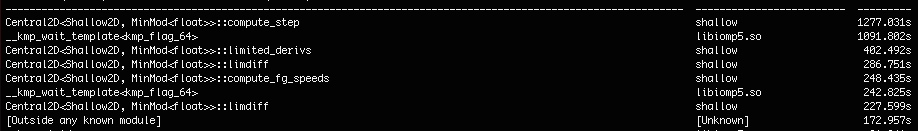
\includegraphics[width=0.7\columnwidth]{naive_omp}
				\caption{Timing of entire simulation using naive implementation of OpenMP parallelized for-loops. Generated using Intel's VTUNE on Totient and recorded in core-seconds.}
				\label{naive_omp}
			\end{center}
		\end{figure}
		
		\subsection{OpenMP for with \texttt{collapse}}
		``OpenMP parallel for'' also has the \texttt{collapse} option, which essentially informs OpenMP how many nested loops are present. By knowing this, OpenMP is able to section both loops to run on multiple processors, creating blocks for each processor to work on. Results when using \texttt{collapse} can be seen in Figure ~\ref{collapse_omp}. It should be noted that the time shown is the total processor time spent and not the per processor time. It was found that using the \texttt{collapse} option actually led to worse performance. We believe this is due to the creation of blocks, which will limit the amount of memory accesses each core has that is of unit stride. When only sectioning the for loops based on the vertical (y) direction, each processor gets a $n \times nx$ block of the array, where $n$ is some number of rows (vertical lines of computational cells) in the domain. This increases memory access locality, which in turn increases cache hits.
			
%		! Will include rest of part on how it performed worse. Need to run 'big' simulation.
			
		\begin{figure}[h]
			\begin{center}
				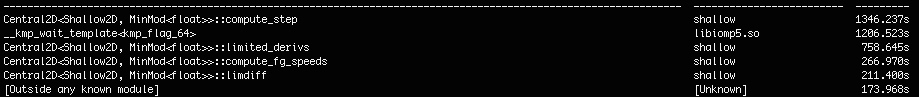
\includegraphics[width=0.7\columnwidth]{collapse_omp}
				\caption{Timing of entire simulation using implementation of OpenMP parallelized for-loops with \texttt{collapse} option. Generated using Intel's VTUNE on Totient and recorded in core-seconds.}
				\label{collapse_omp}
			\end{center}
		\end{figure}
		
		\subsection{OpenMP thread creation limited:}
		
		The constant creation of threads creates a large overhead cost that negatively affects the performance of the program. Therefore, the fewer times that a pool of threads needs to be created the better. In the previous examples, the thread pools were created each time a parallel for loop was called. In order to reduce this costly operation, a pool of threads was only  created within the main run function as shown in the below code section.
		
		\begin{verbatim}
	    for (int io = 0; io < 2; ++io) {
            real cx, cy;
            #pragma omp parallel
            {
            apply_periodic();
            compute_fg_speeds(cx, cy);
            limited_derivs();
            #pragma omp single
                {
            if (io == 0) {
                dt = cfl / std::max(cx/dx, cy/dy);
                if (t + 2*dt >= tfinal) {
                    dt = (tfinal-t)/2;
                    done = true;
                }
            }
                }
            compute_step(io, dt);
            #pragma omp single
            t += dt;
            }

		\end{verbatim}
		
		\noindent Sections of the code that only required one thread to execute took advantage of the omp single pragma command which tells only one thread to run that section of code while the rest wait for it to finish. Inside each of the computation calls the regular omp for pragma command is used to parallelize the various for loops being run. The performance of this operation for the top five costliest function calls when run on the big simulation can be found in Figure ~\ref{ThreadMovement}.
		
		\begin{figure}[h!]
			\begin{center}
				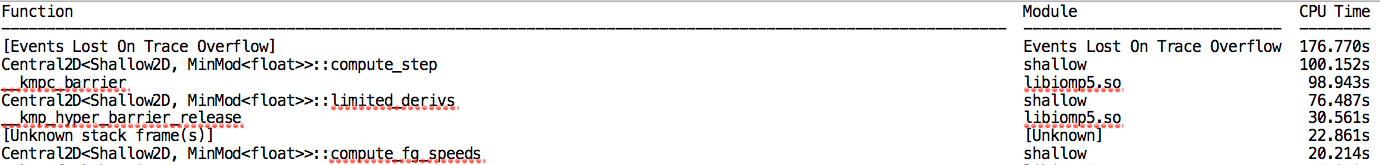
\includegraphics[width=0.8\columnwidth]{ThreadMovement}
				\caption{Timing of five costliest functions using fewer thread creation events. Generated using Intel's VTUNE on Totient.}
				\label{ThreadMovement}
			\end{center}
		\end{figure}
		
		\noindent It should also be noted that these results do include the effects of attempting to force the compiler to vectorize several loops by replacing the min and max calls with an equivalent if statement min and max code. Also from Figure ~\ref{ThreadMovement}, it can be seen that the program still spends a large amount of time in block operations. Based on Figure ~\ref{naive_omp}, it appears that the main cost of thread creation is no longer one of the top performance issues with the code. Now, the internal barrier times is of much more concern.
		
		\subsection{OpenMP nowait implementation:}
		When using the \texttt{omp for} pragma command, an implicit barrier is placed at the end of the loops. Due to the nature of this program, it is possible in several places to be able to assume that a barrier is not needed, and therefore the \texttt{nowait} pragma command can be used. The nowait command could be safely used in the \texttt{compute\_fg\_speeds} and \texttt{limited\_derivs} functions. Then it could be partially used in the \texttt{compute\_step} function once the predictor step was calculated. If the nowait command was used for the predictor loop, synchronization issues are possible when a thread is able to go onto the corrector step while other threads are still in the predictor step. The performance of this implementation for the top five costliest function calls when run on the ``big'' simulation can be found in Figure~\ref{bindoff}
		
		\begin{figure}[h]
			\begin{center}
				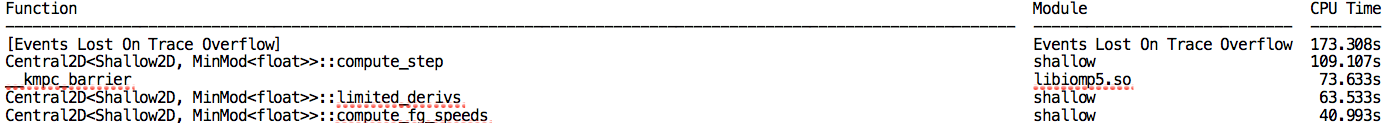
\includegraphics[width=0.8\columnwidth]{bindoff}
				\caption{Timing of five costliest functions using \texttt{nowait} pragma command. Generated using Intel's VTUNE on Totient.}
				\label{bindoff}
			\end{center}
		\end{figure}
		
		\noindent It can be seen by comparing Figure~\ref{ThreadMovement} and Figure~\ref{bindoff} that the overall time spent in the barrier function call has gone down drastically by including the nowait call.
		
		\subsection{Thread Affinity:}
		OpenMP 4.0 offers the ability to describe the ordering of the threads among the CPUs/MICs. Threads can be placed near each other on the same CPU using the OpenMP pragma command \texttt{proc\_bind(close)}. The benefit of doing this is that amount of time for synchronization between threads should decrease. The downside of this is that the available cache and bandwidth per thread will decrease. Another option available distributes the threads more evenly throughout the available CPUs/MIC, and it can be turned on using the OpenMP pragma command \texttt{proc\_bind(spread)}. It should lead to the opposite effects of the close command. The thread affinity was implemented on the code base that used the \texttt{nowait} pragma command. The performance of this implementation for the top five costliest function calls when run on the big simulation can be found in Figure ~\ref{nowait} and Figure ~\ref{nowait2} for the \texttt{proc\_bind(close)} pragma command. Due to system traffic, timing can vary across multiple runs. For this reason, two figures were shown so some measure of variance could be judged. The results for the \texttt{proc\_bind(spread)} command can be found in Figure ~\ref{bindspread}.
		
		\begin{figure}[h]
			\begin{center}
				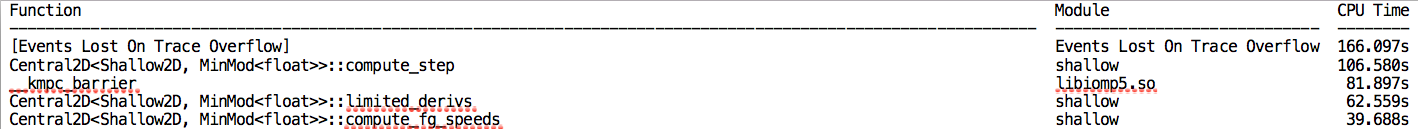
\includegraphics[width=0.8\columnwidth]{nowait}
				\caption{Timing of five costliest functions using \texttt{proc\_bind(close)} pragma command for run 1. Generated using Intel's VTUNE on Totient.}
				\label{nowait}
			\end{center}
		\end{figure}
		
		\begin{figure}[h]
			\begin{center}
				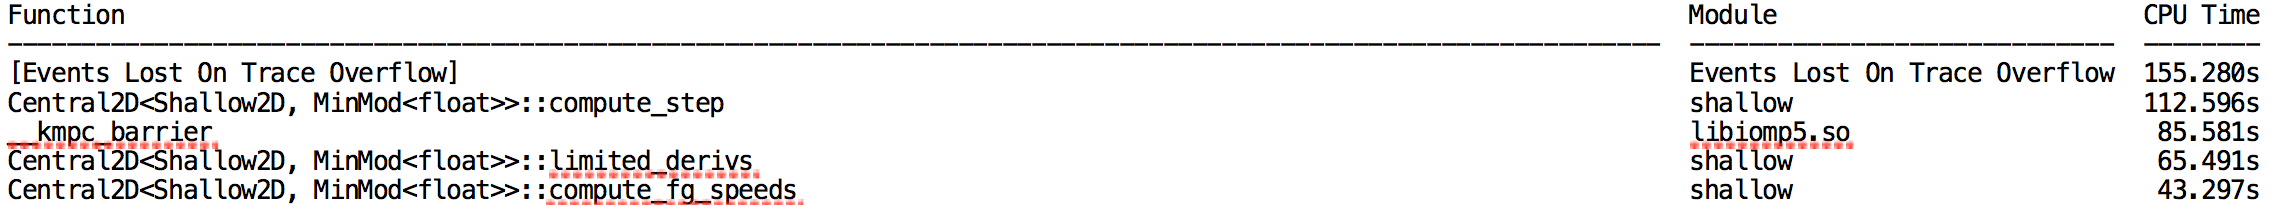
\includegraphics[width=0.8\columnwidth]{nowait2}
				\caption{Timing of five costliest functions using \texttt{proc\_bind(close)} pragma command for run 2. Generated using Intel's VTUNE on Totient.}
				\label{nowait2}
			\end{center}
		\end{figure}
		
		\begin{figure}[h]
			\begin{center}
				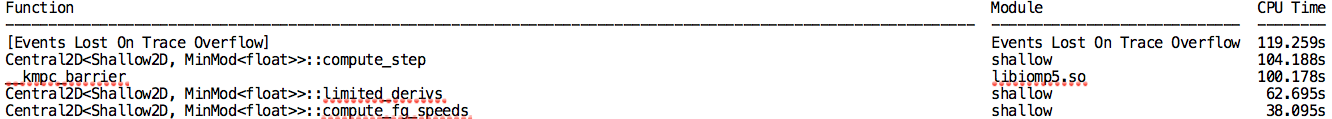
\includegraphics[width=0.8\columnwidth]{bindspread}
				\caption{Timing of five costliest functions using \texttt{proc\_bind(spread)} pragma command. Generated using Intel's VTUNE on Totient.}
				\label{bindspread}
			\end{center}
		\end{figure}
		
		\noindent Overall, both thread affinity options have shown to lead to decreased performance. Therefore, they will not be used in the production code.
		
\section{Analysis}
The current implementation, while offering a sizable speed up over the strictly serial version, still leads much to be desired. Since it currently depends on the \texttt{parallel for} command to run with OpenMP automating certain commands, barriers are automatically placed into the code that limits how each processor accesses the memory of the variables. Further improvements can be made to the code by eliminating these blocking structures where allowed and only syncing the data when the need arises in order to reduce the amount of overhead costs that occur from this type of synchronization. One such place where this could be beneficial is in the \texttt{compute\_step} function. Specific structures could be used in order to ensure the predictor step is done for edge cases before the corrector loop begins without requiring a barrier. To do this, a more rigorous implementation of OpenMP will need to be done, which mimics more of a distributed memory parallel code. Blocks will be made of the domain, where each subdomain has ghost cells and is unaware of what happens outside of itself (except through the ghost cells). This gives more control and limits necessary communication.

\subsection{Strong and Weak Scaling}
The current version of the code can be analyzed for its strong and weak scaling capabilities. The strong scaling will be tested using the ``big'' wave test case with 1000 points in each direction and 100 time steps between frames. The results can be seen in Table~\ref{sstable}. This is tested on the main Xeon chips. With the highest number of threads tested being 16, inter-node communication costs were avoided. VTUNE analysis was also not collected in order to remove any additional time the collection process takes. In Table~\ref{strongscale}, strong scaling is defined by Eq.~\ref{strongscale} and strong scaling efficiency is defined by Eq.~\ref{normss}.

\begin{equation}
\mathrm{Strong \; Scaling} = \frac{t_{\mathrm{serial}}}{t_{\mathrm{parallel}}}
\label{strongscale}
\end{equation}

\begin{equation}
\mathrm{Strong \; Scaling \; Efficiency} = \frac{t_{\mathrm{serial}}}{t_{\mathrm{parallel}}} \frac{1}{p}
\label{normss}
\end{equation}
where $t_{\mathrm{serial}}$ and $t_{\mathrm{parallel}}$ are the times taken when running in serial or parallel, respectively, and $p$ is the number of processors. The strong scaling efficiency is essentially what percentage of perfect linear scaling is actually achieved. This is plotted in Figure~\ref{ssplot}.

\begin{table}[h]
	\begin{center}
		\begin{tabular}{|c c c c|}
			\hline
			Threads & Total Time (seconds) & Strong Scaling & Strong Scaling Efficiency \\ \hline
			1 & 539 & 1.0  & 100\% \\ \hline
			2 & 288 & 1.87 &  93.5\% \\ \hline
			4 & 218 &  2.47&  61.7\%  \\ \hline
			8 & 198 &  2.72&  34.0\%  \\ \hline
			16 & 188 &  2.87& 17.9\%   \\ \hline
		\end{tabular}
		\caption{Strong scaling for wave simulation with 1000 mesh points in each direction and 100 timesteps between frames.}
		\label{sstable}
	\end{center}
\end{table}

		\begin{figure}[h]
			\begin{center}
				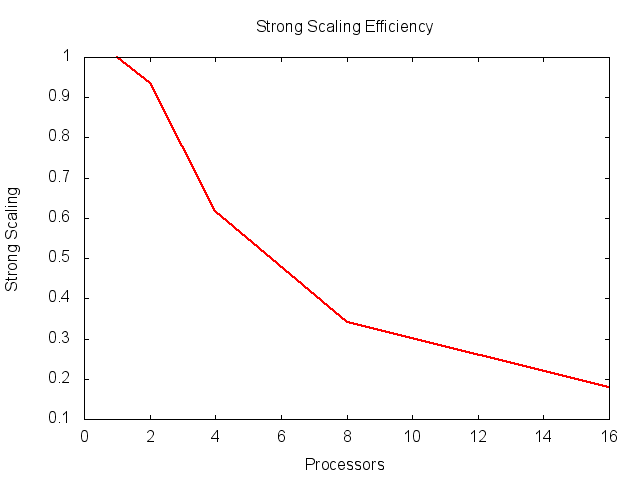
\includegraphics[width=0.5\columnwidth]{ssplot}
				\caption{Plot of strong scaling, representing the data shown in Table~\ref{sstable}.}
				\label{ssplot}
			\end{center}
		\end{figure}

For weak scaling, three simulations were performed, scaling the number of processors equally with the number of cells. The results can be seen in Table~\ref{wstable}. Here, weak scaling is defined by Eq.~\ref{ws}. It was decided to double the side length for each simulation in order to perform the weak scaling test, meaning the number of processors needed to be quadrupled for each run. A plot of the weak scaling can also be seen in Figure~\ref{wsplot}. A more thorough weak scaling test is planned for the future.

\begin{equation}
\mathrm{Weak \; Scaling} = \frac{t_{\mathrm{serial}}(n(p))}{t_{\mathrm{parallel}}(n(p),p)}
\label{ws}
\end{equation}

\begin{table}[h]
	\begin{center}
		\begin{tabular}{|c c c c|}
			\hline
			Threads & Cells Per Side & Total Time (seconds) & Weak Scaling \\ \hline
			1 & 200 & 4.0 & 1.00   \\ \hline
			4 & 400 & 8.3 & 0.485 \\ \hline
			16 & 800 & 73.5 & 0.0544   \\ \hline
		\end{tabular}
		\caption{Weak scaling for wave simulation with 1000 mesh points in each direction and 100 timesteps between frames.}
		\label{wstable}
	\end{center}
\end{table}

		\begin{figure}[h]
			\begin{center}
				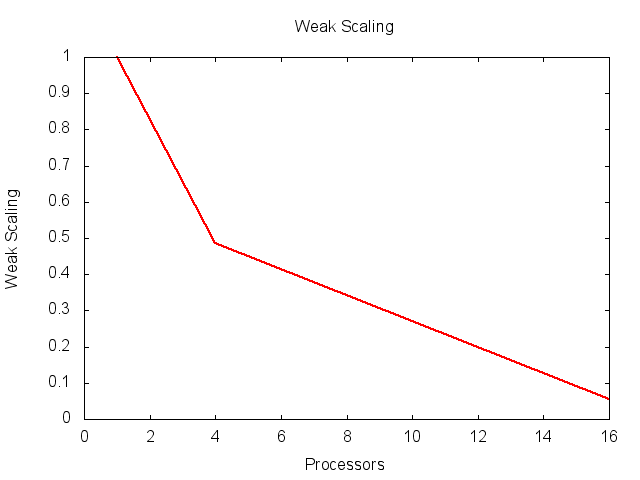
\includegraphics[width=0.5\columnwidth]{wsplot}
				\caption{Plot of weak scaling, representing the data shown in Table~\ref{wstable}.}
				\label{wsplot}
			\end{center}
		\end{figure}

We believe the weak scaling performance is very poor due to our implementation of OpenMP. Weak scaling usually tests the importance of communication on distributed memory systems, since each processor should be performing the same amount of algorithmic work as it is in the serial case. The main difference is the size of data being communicated is largely increased with the scaling in problem size. Since this is a shared memory code, we believe this indicates poor memory handling, leading to many cache misses. This is especially evident in the largest case, where we believe the problem size exceeded the cache size, causes very poor memory use. This could be fixed by a blocking scheme, where the domain is decomposed into subdomains, in order to increase memory locality, reducing the number of cache misses substantially. Another possible reason for the poor performance of the 16 thread case is an increase in time for each communication, due to the threads existing on two separate chips.

The scaling can be represented theoretically by creating an equation for the parallel time taken in the code. This would be primarily made up of two parts: the time to perform the floating point operations, and the portion spent communicating and synchronizing. In this code, since it uses shared memory, the only communications required involves OpenMP barriers and informing each processor of their section of the ``for loops''. These communications will be incorporated into the relation using the variable $t_c$. Predicting the value of $t_c$ consistently is difficult due to uncertainty in how long processors will be required to wait at a barrier. Through running simulations with various parameters, it may be possible to get a rough estimate of the communication time per processor, which could then be used in this model to approximate the scaling for a specific simulation. 

The expression for time taken to execute the simulation in parallel can be represented by Eq.~\ref{part}.

\begin{equation}
t_{\mathrm{parallel}} = \frac{t_{\mathrm{serial}}}{p} + p t_c
\label{part}
\end{equation}

This equation assumes that the serial work will be evenly distributed among all processors, leading to the serial work being completed in $t_{\mathrm{serial}}/p$ time. The cost of parallelizing the code per processor, in the form of communication, barriers, and synchronization, is represented by $t_c$. With an expression for the parallel time, it is now possible to create a rough approximation for scaling, shown in Eq.~\ref{exps}. The difference in strong and weak scaling appears in the values used for $t_{\mathrm{serial}}$ and $t_c$.

\begin{equation}
\mathrm{Scaling} \approx \frac{t_{\mathrm{serial}}}{t_{\mathrm{parallel}}} = \frac{t_{\mathrm{serial}}}{\frac{t_{\mathrm{serial}}}{p} + p t_c} = \left (\frac{1}{p}+p \frac{t_c}{t_{\mathrm{serial}}} \right)^{-1}
\label{exps}
\end{equation}

\newpage
\section{Post Initial Report Work}

\subsection{Swapping of Programming Languages}

Due to the problems that the layer of abstraction within the C++ code base gave the compiler, it was decided it would be best to transition over to Professor Bindel's C version of the code. The C code, when taken, was performing at the same level of performance as the parallelized C++ code when using 16+ threads.  Therefore, this code base will provide an appropriate environment to see what effects various forms of parallelization can have on the performance on the code. Additionally, some more tuning and memory alignment were added to the C version of the code.

\subsection{Vectorization and other optimizations of the code base}

While the C code is rather vectorized, it still had a couple of areas of improvement that could be made to allow the compiler to better vectorize the various loops in the code. First off, the various techniques used in the matmul assignment can be introduced here including aligning the memory to a 32 byte boundary and the use of the \texttt{\# pragma vector aligned} command. The \texttt{\_mm\_malloc()} and \texttt{\_mm\_free()} commands were used in place of the \texttt{malloc} and \texttt{free} commands for the creation of the \texttt{sim} and \texttt{sim->u} variables. This allowed the compiler to know that these variables would be aligned to a 32 byte boundary. Also since several other variables are based upon the \texttt{sim->u}, the compiler recognizes that these also should be aligned to a 32 byte boundary as well. Next, the \texttt{\# pragma vector aligned} is used at each for loop used in both the stepper.c and shallow2d.c files. Since all the vector variables with initial data have been aligned, the various calculations done inside the loop will not lead to a segmentation fault. If this was not the case, the \texttt{\_\_attribute\_\_((aligned( 32 )))} would need to be used during the declaration of those variables in order to ensure those variables were aligned. It should also be noted that if the Xeon Phi chips were being used, then the vectors could be aligned to a 64 byte boundary instead, since the chip set supports the AVX512 instruction set. Finally, the following Intel compiler optimization flags were used to ensure we are taking full advantage of the Xeon architecture during our vectorization attempts:\texttt{-O3 -axcore-avx2 -march=core-avx2 -unroll-aggressive -m64 -ipo -no-prec-div -ansi-alias}. \\

Next, there are several places where the same variable is created and assigned inside a for loop. This constant creation of these variables lead to a slow down of the code. Therefore, if the variable being created did not call for the use of the const or restrict keywords it was initially created outside of the loop(s). This move was done for both the stepper.c and shallow2d.c file. The results when comparing the baseline C code, and the further optimized code can be seen in Table ~\ref{opttable} for a 1000x1000 size mesh. It can be seen while the speed up is minor, it does provide some improvement on an already well optimized code base.

\begin{table}[h]
	\begin{center}
		\begin{tabular}{|c c c|}
			\hline
			Simulation Name & Time(s) & Speed up(\%) \\ \hline
			Baseline Code & 59.8 & 100   \\ \hline
			Aligned Code & 55.9 & 107 \\ \hline
		\end{tabular}
		\caption{Comparison of baseline and aligned C code bases for a simulation with 1000 mesh points and 50 frames.}
		\label{opttable}
	\end{center}
\end{table}



\subsection{Naive OpenMP Implementation}
A naive OpenMP implementation was used initially in this code base where no subdomain blocking has yet to be implemented. The purpose of this is to see what effects parallelization techniques will have on an already fairly well optimized code base with good performance. The OpenMP implementation will be based upon the best implementation used in the C++ code base, initially presented above in the first submission. Although, one of the major differences will be that the user can now directly specify the number of threads to use when the program runs. The main shallow2d run function now looks like the following:

\begin{verbatim}
omp_set_num_threads(p); \\where p is the number of threads being used
        #pragma omp parallel
        {
        #pragma omp single
        {
        central2d_periodic(u, nx, ny, ng, nfield);
        speed(cxy, u, nx_all * ny_all, nx_all * ny_all);

        dt = cfl / fmaxf(cxy[0]/dx, cxy[1]/dy);
        if (t + 2*dt >= tfinal) {
            dt = (tfinal-t)/2;
            done = true;
        }
        }
        central2d_step(u, v, scratch, f, g,
                       0, nx+4, ny+4, ng-2,
                       nfield, flux, speed,
                       dt, dx, dy);
        central2d_step(v, u, scratch, f, g,
                       1, nx, ny, ng,
                       nfield, flux, speed,
                       dt, dx, dy);
        #pragma omp single
        {
        t += 2*dt;
        nstep += 2;
        }
        }
\end{verbatim}

It was then found that the following functions could contain a parallelized for loop: central2d\_step, central2d\_correct\_sd, limited\_deriv1, and limited\_derivk. The various other functions contained in here, if parallelized, would lead to negative height being seen. Also, it should be noted that loop counter variable needed to be declared outside the loop and then declared private for the C code. The actual results of implementing this will be seen in the weak and strong scaling subsection, but it should be noted that this implementation resulted in a vastly slower performance. It needs to also be noted that when the mesh becomes more refined an increase in threads will lead to a height less than 0 assertion to happen. This was discovered when trying to run the weak scaling study. One explanation could be that a nonintuitive race condition is occurring that is allowing one thread change the value of variable that another thread has yet to use. However, the OpenMP implementation of a barrier at the end of each for loop should prevent this from occurring, although leading to a degradation in performance.

\subsection{Weak and Strong Scaling for Tuned C Code}

The strong scaling for the naive OpenMP implementation can be seen in Table ~\ref{sscale_c} and Figure ~\ref{ssplot_c}. It can be seen that the parallelization has led to a degradation in performance and this can be mainly contributed to the communication cost between threads. Also, it is not as large of a factor anymore the constant creation of threads is also a problem. One thing that should also be noted is that since a less than 0 assertion can be reached for larger mesh sizes the strong scaling done for the C code base is not identical to the one performed previously for the C++ code base.

\begin{table}[h]
	\begin{center}
		\begin{tabular}{|c c c c|}
			\hline
			Threads & Total Time (seconds) & Strong Scaling & Strong Scaling Efficiency(\%) \\ \hline
			1 & 2.39 & 1.00  & 100.0 \\ \hline
			2 & 11.40 & 0.21 &  10.0 \\ \hline
			4 & 20.71 &  0.12&  3.0  \\ \hline
			8 & 25.03 &  0.10&  1.0  \\ \hline
			16 & 31.13 &  0.08& 0.5   \\ \hline
		\end{tabular}
		\caption{Strong scaling for wave simulation with 400 mesh points in each direction and 50 timesteps between frames.}
		\label{sscale_c}
	\end{center}
\end{table}

		\begin{figure}[h]
			\begin{center}
				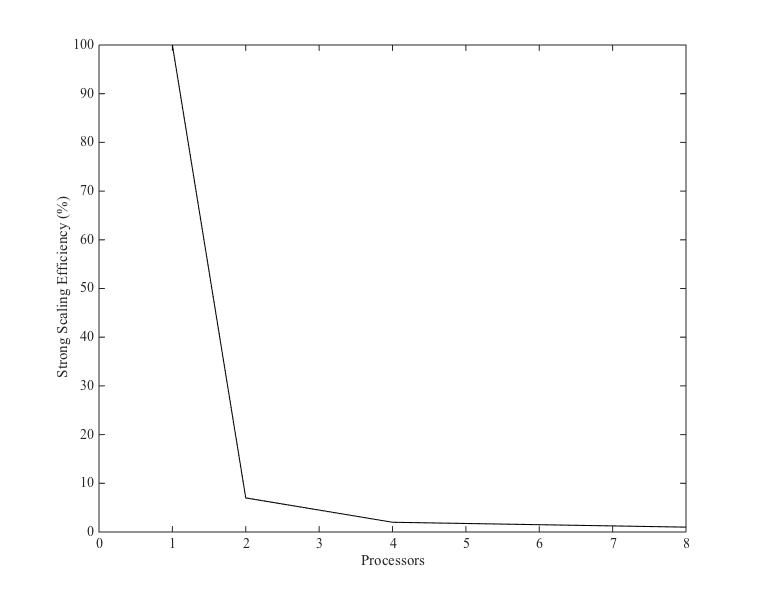
\includegraphics[width=0.5\columnwidth]{sscale_plot}
				\caption{Plot of strong scaling, representing the data shown in Table~\ref{sscale_c}.}
				\label{ssplot_c}
			\end{center}
		\end{figure}

Next, the weak scaling can be seen in Table ~\ref{wscale_c} and Figure ~\ref{wsplot_c}. A couple more points were obtained for this study by taking a $\sqrt{2}$ increase in cell size in order to be able to double the number of threads. It can also be seen from this table that the naive implementation of OpenMP had detrimental effects on the performance of the code.

\begin{table}[h]
	\begin{center}
		\begin{tabular}{|c c c c|}
			\hline
			Threads & Cells Per Side & Total Time (seconds) & Weak Scaling(\%) \\ \hline
			1 & 200 & 0.35 & 100   \\ \hline
			2 & 283 & 5.11 & 7 \\ \hline
			4 & 400 & 17.70 & 2   \\ \hline
			8 & 566 & 55.61 & 1   \\ \hline
		\end{tabular}
		\caption{Weak scaling for wave simulation with 50 frames and N varying mesh size.}
		\label{wscale_c}
	\end{center}
\end{table}

		\begin{figure}[h]
			\begin{center}
				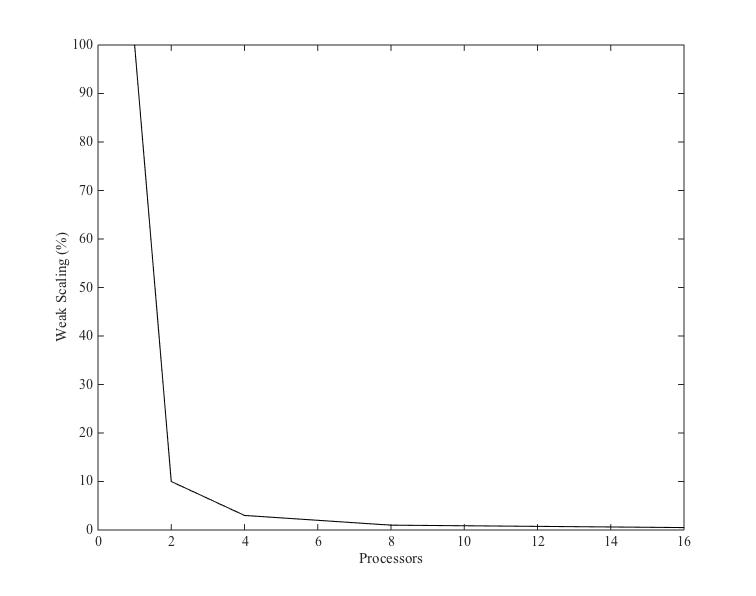
\includegraphics[width=0.5\columnwidth]{wscale_plot}
				\caption{Plot of weak scaling, representing the data shown in Table~\ref{wscale_c}.}
				\label{wsplot_c}
			\end{center}
		\end{figure}

It can be seen from these scalings that in order to even attempt at getting better performance out of the code a subdomain implementation of OpenMP will need to be used. This was done separately from these tuning improvements due to time constraints and is preented next.

\subsection{Parallelization}
The C code was explicitly decomposed into subdomains using OpenMP with a distributed memory type paradigm. In \texttt{ldriver.c}, a thread team is launched that decomposes the domain by \texttt{npx} processors in the x-direction and \texttt{npy} processors in the y-direction, where \texttt{npx} and \texttt{npy} can be set by the lua script. It is required in the code, however, that the size of the domain be evenly divisible by the number of processors. Once the thread team is launched, the location of the subdomain on the global domain is noted for each processor for easy copying to the global domain. After this point, each subdomain is not aware of the others and the simulation is effectively distributed memory. For exchanging information between threads and informing the ghost cells, the global domain is used. Communication is handled as followed. While in the flow solver, boundary cell values are pushed to their correct location on the global domain. Next, one processor runs the original periodic boundary condition function. Then, each subdomain fills its ghost cells using the global domain. This is not the most efficient method due to the barriers required while one processor performs the periodic boundary condition update on the global domain, however provided easy implementation. The one other quantity communicated between the processors is the time step, used to restrict the time step each processor used to the most stringent time step in the entire global domain. This required large modifications to the \texttt{central2d\_t} structure and other portions of the code. The modified code can be seen in the \texttt{dist\_par} subdirectory of the git repository. As shown below, significant improvements in strong and weak scaling were gained when compared to a naive OpenMP parallel-for implementation.

\subsubsection{Strong and Weak Scaling}
The strong and weak scaling for this parallelization can also be analyzed as before. Although it will not be a direct comparison to the study done using the naive OpenMP implementation and more tuned C code, the same running parameters will be used, allowing some small comparison. The strong scaling study was run for a simulation with 400 mesh points per side and 50 frames, the results of which can be seen in Table~\ref{sscale_c_dist} and Figure~\ref{ssplot_c_dist}. Strong scaling was once again calculated using Eq.~\ref{strongscale}, with the normalized strong scaling calculated with Eq.~\ref{normss}.

\begin{table}[h]
	\begin{center}
		\begin{tabular}{|c c c c|}
			\hline
			Threads & Total Time (seconds) & Strong Scaling & Strong Scaling Efficiency(\%) \\ \hline
			1 & 5.974 & 1.00  & 100.0 \\ \hline
			2 & 3.272 & 1.82 &  91.0 \\ \hline
			4 & 1.695 &  3.52&  88.0  \\ \hline
			8 & 0.9780 &  6.11&  76.4  \\ \hline
			16 & 0.8821 & 6.77 &  42.3 \\ \hline
		\end{tabular}
		\caption{Strong scaling for wave simulation with 400 mesh points in each direction and 50 timesteps between frames using distributed memory paradigm.}
		\label{sscale_c_dist}
	\end{center}
\end{table}

\begin{figure}[h]
	\begin{center}
		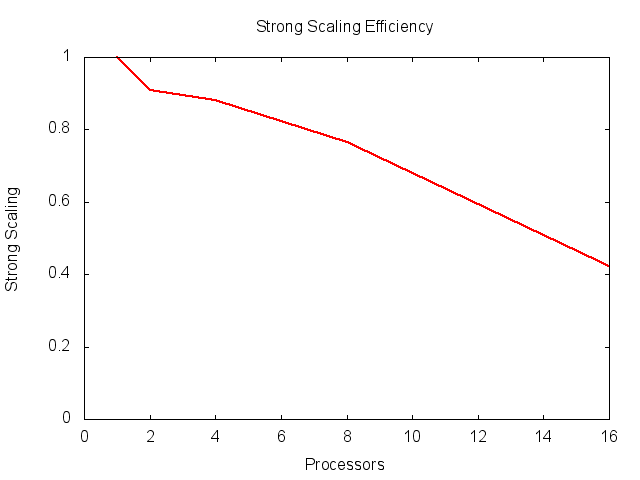
\includegraphics[width=0.5\columnwidth]{ssplot_c_dist}
		\caption{Plot of strong scaling, representing the data shown in Table~\ref{sscale_c_dist}.}
		\label{ssplot_c_dist}
	\end{center}
\end{figure}

There are three important facts to note from the strong scaling study. First, running this parallelized version with one processor (in serial) is a little less than three times slower than the tuned version of C we also presented. This is most likely due to the more complicated boundary condition handling and the existence of two grids, even when running the parallel code in serial. Second, the strong scaling shown here for this parallelized C version performs much better than the naively OpenMP parallelized version. This is due to the separation of the thread team during the driver stage and limited communication afterwards. Third, There is a stark degradation in strong scaling between 8 processors and 16 processors. This is most likely due to the fact that the processors used now exist on two separate chips on the node. This will significantly increase communication costs which will impact performance, as seen in Table~\ref{sscale_c_dist}. 

Similarly, a weak scaling study can also be performed. This is shown in Table~\ref{wscale_c_dist} and Figure~\ref{wsplot_c_dist}. Weak scaling was once again calculated using Eq.~\ref{ws}.


\begin{table}[h]
	\begin{center}
		\begin{tabular}{|c c c c|}
			\hline
			Threads & Cells Per Side & Total Time (seconds) & Weak Scaling(\%) \\ \hline
			1 & 200 & 0.8876 & 100.0   \\ \hline
			2 & 284 & 1.308 &  67.9 \\ \hline
			4 & 400 & 1.708 &  52.0   \\ \hline
			8 & 566 & 2.655 & 33.4   \\ \hline
		\end{tabular}
		\caption{Weak scaling for wave simulation with 50 frames and N varying mesh size using distributed memory paradigm.}
		\label{wscale_c_dist}
	\end{center}
\end{table}

\begin{figure}[h]
	\begin{center}
		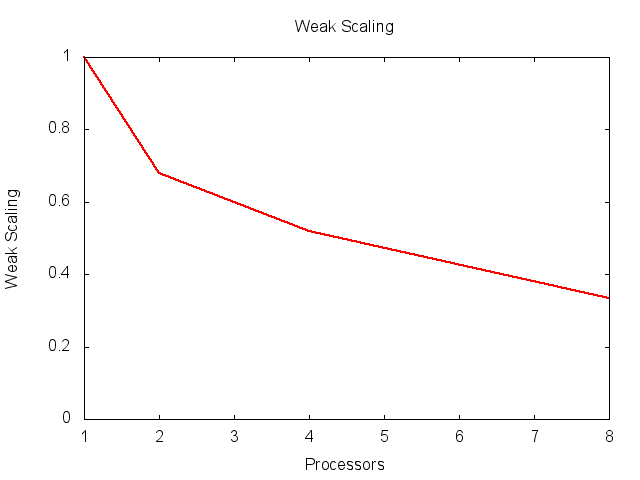
\includegraphics[width=0.5\columnwidth]{wsplot_c_dist}
		\caption{Plot of weak scaling, representing the data shown in Table~\ref{wscale_c_dist}.}
		\label{wsplot_c_dist}
	\end{center}
\end{figure}
Once again, the weak scaling with this parallelization method proves to be much more effective than the naively implemented OpenMP parallelized code used on the tuned C code. This is due to the much lower communication and synchronization in this parallelization method as opposed to the naive OpenMP implementation. Please note, the number of cells per side were slightly modified to make them evenly divisible by the number of processors for that side, a requirement of this parallelization method.


\section{Possible Future Work and Improvements}
There are several remaining ways the code could be improved. First, the tuned improvements and the distributed memory type paradigm we used to parallelize the code could be combined to achieve even greater speed. For the parallel method itself, the communication between processors and handling of the periodic boundary condition could be changed, so that one OpenMP barrier and the OpenMP single command could be removed, increasing load balance and decreasing synchronization time. Lastly, while not in the flow solver itself, the exporting of visualization quantities could be parallelized, once again increasing load balancing and removing the need to copy the entire subdomains onto the global domain.

After these improvements, the next logical progression of work would be to offload work to the Xeon Phi's, allowing even greater parallelization. When doing this, however, the memory usage would need to be considered due to the limited memory per processor. A blocking scheme could be used, where the domain is first split into subdomains that will fit into the L2 cache for each processor. Then, one or more of these smaller blocks could be assigned to each processor, ensuring cache locality and maintaining strong parallelization.




%\FloatBarrier
%	\bibliography{report.bib} 
%	\bibliographystyle{unsrt}
	
\end{document}